\index{Essential Boundary Conditions}
\index{Natural Boundary Conditions}

Boundary conditions come in two basic flavors: essential and natural.
\begin{itemize}
\item Essential bcs directly affect DOFs, and are imposed on the FEM matrix. 
\item Natural bcs do not directly affect DOFs and are imposed on the right-hand side vector.
\end{itemize}

\subsubsection{In-out flux boundary conditions for lithospheric models}

\begin{center}
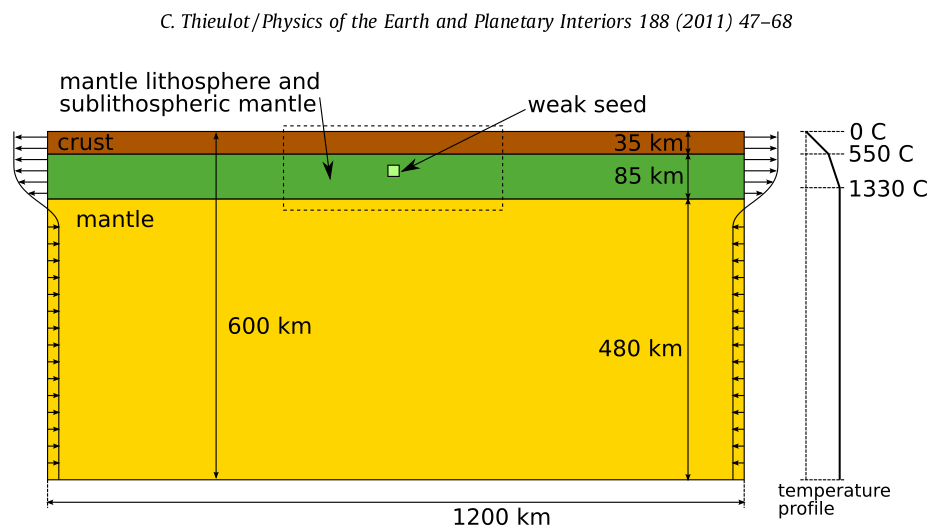
\includegraphics[width=8cm]{images/boundary_conditions/bc1}\\
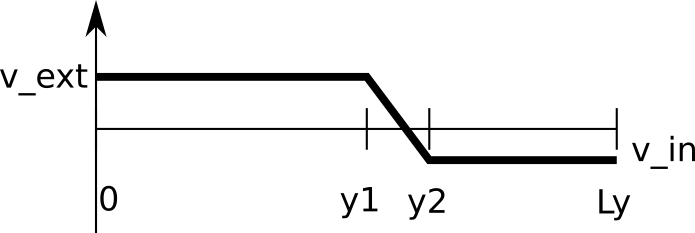
\includegraphics[width=8cm]{images/boundary_conditions/drawing.png}
\end{center}

The velocity on the side is given by
\begin{eqnarray}
u(y) &=& v_{ext} \quad\quad y<L_1 \nn\\
u(y) &=& \frac{v_{in}-v_{ext}}{y_2-y_1}(y-y_1) + v_{ext} \quad\quad y_1<y<y_2 \nn\\
u(y) &=& v_{in} \quad\quad y>y_2 \nn
\end{eqnarray}
The requirement for volume conservation is:
\[
\Phi=\int_{0}^{L_y} u(y) dy = 0
\]
Having chosen $v_{in}$ (the velocity of the plate), one can then compute $v_{ext}$
as a function of $y_1$ and $y_2$.

\begin{eqnarray}
\Phi
&=&\int_{0}^{y_1} u(y) dy  +\int_{y_1}^{y_2} u(y) dy +\int_{y_2}^{L_y} u(y) dy \nn\\
&=& v_{ext} y_1  + \frac{1}{2}(v_{in}+v_{ext})(y_2-y_1) + (L_y-y_2) v_{in} \nn\\
&=& v_{ext} [y_1 + \frac{1}{2}(y_2-y_1) ] + v_{in} [ \frac{1}{2}(y_2-y_1)  + (L_y-y_2) ] \nn\\
&=& v_{ext}\frac{1}{2} (y_1 + y_2 ) + v_{in} [ L_y - \frac{1}{2}(y_1+y_1) ] \nn
\end{eqnarray}
and finally
\[
v_{ext} = -v_{in} \frac{ L_y - \frac{1}{2}(y_1+y_1)}{ \frac{1}{2} (y_1 + y_2 ) }
\]
